\documentclass[11pt,a4paper]{article}

% ---- Packages ----
\usepackage[margin=1in]{geometry}
\usepackage{graphicx}
\usepackage{amsmath,amssymb}
\usepackage{booktabs}
\usepackage{hyperref}
\usepackage{float}
\usepackage{caption}
\usepackage{subcaption}
\usepackage{listings}
\usepackage{xcolor}
\usepackage{enumitem}
\usepackage{multirow}

% ---- Figure paths ----
\graphicspath{
  {../Final-Presentation/final-project/comparison_plots/comparison_plots/}
  {../Final-Presentation/final-project/models/baseline_cnn/plots/}
  {../Final-Presentation/final-project/models/Weight-Focus/plots/}
  {../Final-Presentation/final-project/models/MoE/plots/}
}

% ---- Code listing style ----
\lstdefinestyle{pythonstyle}{
  language=Python,
  basicstyle=\ttfamily\footnotesize,
  keywordstyle=\color{blue}\bfseries,
  commentstyle=\color{gray}\itshape,
  stringstyle=\color{red},
  showstringspaces=false,
  breaklines=true,
  frame=single,
  numbers=left,
  numberstyle=\tiny\color{gray},
  tabsize=4,
  captionpos=b,
}
\lstset{style=pythonstyle}

% ---- Title ----
\title{%
  \textbf{Predicting Nutritional Content from Food Images\\Using Deep Multi-Task Regression}\\[0.5em]
  \large Deep Learning --- Spring 2026 Final Project Report
}
\author{Zac Bland}
\date{May 5, 2026}

\begin{document}
\maketitle

% ===========================================================================
% 1. INTRODUCTION
% ===========================================================================
\section{Introduction}

Accurate dietary tracking is essential for health management, weight control, and clinical nutrition, yet manual food logging is tedious and error-prone. This project investigates the use of deep convolutional neural networks to automatically predict the nutritional content of food from images. Specifically, we predict five nutritional outputs---calories, mass (grams), fat (grams), carbohydrates (grams), and protein (grams)---from overhead and side-angle photographs of cafeteria dishes.

Our approach is based on the architecture described in the CVPR 2021 paper by Thames et al.\ \cite{thames2021}, which introduced the Nutrition5k dataset and demonstrated that a convolutional backbone with multi-task regression heads can predict dish-level nutritional content with reasonable accuracy. We use InceptionV3 \cite{szegedy2016} pretrained on ImageNet \cite{deng2009} as our backbone, since the original paper's InceptionV2 backbone pretrained on JFT-300M is not publicly available.

We explore three architectural variants built on this foundation:
\begin{enumerate}
  \item \textbf{Baseline CNN}: A direct implementation of the paper's architecture with shared fully connected layers and independent per-task regression heads.
  \item \textbf{Weight-Focus}: A variant where mass is predicted first, and the mass prediction is fed as an additional input to the remaining nutrient heads, based on the intuition that food mass is correlated with caloric and macronutrient content.
  \item \textbf{Mixture of Experts (MoE)}: A variant that replaces the shared FC layers with a gated mixture of expert networks, allowing the model to learn specialized feature transformations for different types of food.
\end{enumerate}

The remainder of this report is organized as follows: Section~\ref{sec:schedule} presents the project schedule, Section~\ref{sec:dataset} describes the Nutrition5k dataset, Section~\ref{sec:network} details the network architectures and training algorithm, Section~\ref{sec:setup} covers the experimental setup, Section~\ref{sec:results} presents and discusses results, Section~\ref{sec:conclusion} provides conclusions and future work, and Section~\ref{sec:references} lists references. Appendix~\ref{sec:appendix} contains selected code listings.

% ===========================================================================
% 2. PROJECT SCHEDULE
% ===========================================================================
\section{Project Schedule}
\label{sec:schedule}

Table~\ref{tab:schedule} summarizes the project timeline, derived from the Git commit history across the \texttt{main}, \texttt{weight-focus}, and \texttt{MoE} branches.

\begin{table}[H]
\centering
\caption{Project schedule with key milestones (from Git history).}
\label{tab:schedule}
\begin{tabular}{@{}lll@{}}
\toprule
\textbf{Date} & \textbf{Activity} & \textbf{Branch} \\
\midrule
03/26 & \textbf{Proposal submitted}; initial repository commit & \texttt{main} \\
04/15 & Dataset download script; GCS pipeline for Nutrition5k images & \texttt{main} \\
04/16 & Baseline CNN: training/test code, InceptionV3 backbone, & \texttt{main} \\
       & \quad data metadata, aux\_logits fix, training plots, & \\
       & \quad per-nutrient MAE\%, backbone freeze, cosine annealing, & \\
       & \quad augmentations, side-angle pre-flip, dropout/weight decay, & \\
       & \quad early stopping, verify images script & \\
04/17 & Overfitting fixes: sub-sample side frames, label normalization, & \texttt{main} \\
       & \quad stronger regularization; batch size 32; save\_experiment script & \\
\cmidrule(lr){1-3}
04/17 & \textbf{Weight-Focus branch created}: added mass-focused loss & \texttt{weight-focus} \\
       & \quad weighting (3$\times$ mass); mass-conditioned architecture & \\
04/17 & \textbf{MoE branch created}: gating network, 4 expert networks, & \texttt{MoE} \\
       & \quad load-balancing loss & \\
\cmidrule(lr){1-3}
04/20 & Comparative analysis: comparison plots, test.py argparse, & \texttt{main} \\
       & \quad label\_mean in test/train, outlier finder, & \\
       & \quad Weight-Focus test fix & \\
04/24 & \textbf{Final presentation slides} posted to GitHub & \texttt{main} \\
04/28--30 & \textbf{Oral presentations} & --- \\
05/01 & Updated .gitignore; added report directory & \texttt{main} \\
05/05 & \textbf{Final report due} & --- \\
\bottomrule
\end{tabular}
\end{table}

% ===========================================================================
% 3. DESCRIPTION OF THE DATA SET
% ===========================================================================
\section{Description of the Data Set}
\label{sec:dataset}

We use the \textbf{Nutrition5k} dataset introduced by Thames et al.\ \cite{thames2021}, which is publicly available via Google Cloud Storage. The dataset was collected at two Google cafeterias and contains images of real cafeteria dishes paired with precise nutritional labels obtained from the cafeteria's point-of-sale system and ingredient databases.

\subsection{Dataset Statistics}

\begin{itemize}
  \item \textbf{Total dishes}: 5,006 unique dishes across two cafeterias
  \item \textbf{Dishes with overhead images}: $\sim$3,500 (not all metadata entries have corresponding images)
  \item \textbf{Train split}: 4,058 dishes (as defined by the official \texttt{rgb\_train\_ids.txt})
  \item \textbf{Test split}: 708 dishes (as defined by the official \texttt{rgb\_test\_ids.txt})
  \item \textbf{Image types}: Overhead RGB (one per dish) + side-angle video frames from cameras B and C
\end{itemize}

\subsection{Image Sources}

Each dish is photographed from multiple angles:
\begin{itemize}
  \item \textbf{Overhead}: A single top-down RGB image (\texttt{rgb.png}) captured by a RealSense camera mounted above the food tray.
  \item \textbf{Side-angle}: Video frames extracted from two side-mounted cameras (camera\_B and camera\_C). These provide complementary viewpoint information about food height and texture. Side-angle frames are vertically flipped during download to correct their original orientation.
\end{itemize}

Using all three viewpoints (overhead + 2 side cameras), our training set contains 9,409 samples and our validation set contains 5,853 samples.

\subsection{Labels}

Each dish has five numerical labels:
\begin{itemize}
  \item \textbf{Calories} (kcal) --- total caloric content
  \item \textbf{Mass} (g) --- total weight of the dish
  \item \textbf{Fat} (g) --- total fat content
  \item \textbf{Carbohydrates} (g) --- total carbohydrate content
  \item \textbf{Protein} (g) --- total protein content
\end{itemize}

These labels are parsed from \texttt{ingredients\_metadata.csv}, which provides dish-level aggregated nutritional information. The labels span a wide range (e.g., calories range from near-zero to over 2,000 kcal), creating a challenging regression problem.

\subsection{Label Normalization}

Because the five nutritional outputs have very different scales (e.g., calories are typically in the hundreds while protein may be in the tens), we normalize labels during training by dividing each by its mean across the training set. This ensures all task losses contribute equally and prevents any single output from dominating the gradient signal. Predictions are denormalized back to original units for evaluation.

% ===========================================================================
% 4. DESCRIPTION OF THE DEEP LEARNING NETWORK AND TRAINING ALGORITHM
% ===========================================================================
\section{Description of the Deep Learning Network and Training Algorithm}
\label{sec:network}

\subsection{Backbone: InceptionV3}

All three model variants share the same backbone: \textbf{InceptionV3} \cite{szegedy2016} pretrained on ImageNet \cite{deng2009}. InceptionV3 is a deep convolutional network that uses factorized convolutions and aggressive regularization to achieve strong image classification performance while remaining computationally efficient. The network expects $299 \times 299$ RGB input images and produces a 2048-dimensional feature vector after global average pooling.

The original paper \cite{thames2021} used InceptionV2 pretrained on JFT-300M (a proprietary Google dataset of 300 million images). Since JFT-300M is not publicly available, we substitute InceptionV3 pretrained on ImageNet, which provides a strong but publicly accessible initialization.

We replace the final classification layer with an identity function to extract the 2048-dimensional feature representation:
\begin{equation}
  \mathbf{f} = \text{InceptionV3}(\mathbf{x}) \in \mathbb{R}^{2048}
\end{equation}
where $\mathbf{x} \in \mathbb{R}^{3 \times 299 \times 299}$ is the input image.

\subsection{Architecture 1: Baseline CNN}

The baseline architecture follows the paper's design. After the backbone, features pass through two shared fully connected layers, followed by five independent per-task regression heads:

\begin{equation}
  \mathbf{h} = \text{ReLU}(\mathbf{W}_2 \cdot \text{ReLU}(\mathbf{W}_1 \cdot \mathbf{f} + \mathbf{b}_1) + \mathbf{b}_2)
\end{equation}

where $\mathbf{W}_1 \in \mathbb{R}^{4096 \times 2048}$, $\mathbf{W}_2 \in \mathbb{R}^{4096 \times 4096}$, and $\mathbf{h} \in \mathbb{R}^{4096}$ is the shared representation. Each task head $k$ then computes:

\begin{equation}
  \hat{y}_k = \mathbf{w}_k^{(2)} \cdot \text{ReLU}(\mathbf{W}_k^{(1)} \cdot \mathbf{h} + \mathbf{b}_k^{(1)}) + b_k^{(2)}
\end{equation}

where $\mathbf{W}_k^{(1)} \in \mathbb{R}^{4096 \times 4096}$ and $\mathbf{w}_k^{(2)} \in \mathbb{R}^{4096}$. Dropout ($p = 0.6$) is applied after each ReLU activation.

\textbf{Total parameters}: 130,886,629 (109,101,061 trainable after unfreezing backbone).

\subsection{Architecture 2: Weight-Focus}

The Weight-Focus variant is motivated by the observation that food mass (weight) is strongly correlated with caloric and macronutrient content. By predicting mass first and conditioning the remaining predictions on the mass estimate, we hypothesize that the model can better calibrate its nutritional estimates. This variant also uses a \textbf{weighted per-task loss} with \texttt{TASK\_WEIGHTS = [1.0, 3.0, 1.0, 1.0, 1.0]}, giving the mass prediction 3$\times$ the loss weight of other nutrients to prioritize accurate mass estimation.

The architecture is identical to the Baseline through the shared FC layers. The key differences are:
\begin{enumerate}
  \item A dedicated \textbf{mass head} predicts mass first: $\hat{y}_{\text{mass}} = f_{\text{mass}}(\mathbf{h})$
  \item Four \textbf{conditioned heads} for calories, fat, carbs, and protein each receive the shared representation \emph{concatenated} with the mass prediction:
\end{enumerate}
\begin{equation}
  \hat{y}_k = f_k([\mathbf{h}; \hat{y}_{\text{mass}}]) \quad \text{for } k \in \{\text{cal}, \text{fat}, \text{carbs}, \text{protein}\}
\end{equation}

where $[\cdot;\cdot]$ denotes concatenation, resulting in a 4097-dimensional input to each conditioned head (4096 from shared features + 1 from mass prediction).

The weighted per-task loss is computed as:
\begin{equation}
  \mathcal{L}_{\text{WF}} = \frac{1}{N} \sum_{i=1}^{N} \frac{1}{5} \sum_{k=1}^{5} w_k \left| \hat{y}_k^{(i)} - y_k^{(i)} \right|
\end{equation}
where $w_k$ are the task weights ($w_{\text{mass}} = 3.0$, all others $= 1.0$). This ensures the mass head receives a stronger gradient signal, which is critical since the conditioned heads depend on its output.

\textbf{Total parameters}: 130,903,013 (109,117,445 trainable).

\subsection{Architecture 3: Mixture of Experts (MoE)}

The Mixture of Experts variant replaces the shared FC layers with a gated ensemble of specialist sub-networks. The intuition is that different types of food (e.g., soups vs.\ salads vs.\ entrees) may benefit from specialized feature transformations.

The architecture consists of:
\begin{enumerate}
  \item A \textbf{gate network} that produces a probability distribution over $K = 4$ experts:
  \begin{equation}
    \mathbf{g} = \text{softmax}(\mathbf{W}_g \cdot \mathbf{f} + \mathbf{b}_g) \in \mathbb{R}^{4}
  \end{equation}
  \item $K = 4$ \textbf{expert networks}, each a two-layer MLP:
  \begin{equation}
    \mathbf{e}_i = \text{MLP}_i(\mathbf{f}) \in \mathbb{R}^{2048}, \quad i = 1, \ldots, 4
  \end{equation}
  \item The expert outputs are combined via the gate weights:
  \begin{equation}
    \mathbf{h} = \sum_{i=1}^{4} g_i \cdot \mathbf{e}_i
  \end{equation}
  \item Five \textbf{task heads} map from the combined expert representation to scalar predictions:
  \begin{equation}
    \hat{y}_k = f_k(\mathbf{h}), \quad \mathbf{h} \in \mathbb{R}^{2048} \rightarrow \mathbb{R}^{1024} \rightarrow \mathbb{R}^{1}
  \end{equation}
\end{enumerate}

Unlike the other two architectures, the MoE model's \texttt{forward()} method returns a tuple \texttt{(predictions, balance\_loss)}, where the balance loss is an auxiliary regularization term that penalizes uneven expert utilization:
\begin{equation}
  \mathcal{L}_{\text{balance}} = K \sum_{i=1}^{K} \bar{g}_i^2
\end{equation}
where $\bar{g}_i = \frac{1}{N}\sum_{n=1}^{N} g_i^{(n)}$ is the mean gate weight for expert $i$ across the batch. This encourages the gate to distribute inputs across all experts rather than collapsing to a single dominant expert.

\textbf{Total parameters}: 65,860,585 (44,075,017 trainable) --- roughly half the parameters of the other two architectures.

\subsection{Loss Function}

Following the reference paper, we use the \textbf{L1 loss} (Mean Absolute Error) as the base training loss:
\begin{equation}
  \mathcal{L}_{\text{L1}} = \frac{1}{N} \sum_{i=1}^{N} \frac{1}{5} \sum_{k=1}^{5} \left| \hat{y}_k^{(i)} - y_k^{(i)} \right|
\end{equation}
where $\hat{y}_k^{(i)}$ and $y_k^{(i)}$ are the predicted and ground-truth normalized values for nutrient $k$ of sample $i$. L1 loss is preferred over L2 (MSE) because it is more robust to outliers, which are common in food nutrition data (e.g., dishes with unusually high calorie counts).

Each model variant uses a different total loss:
\begin{itemize}
  \item \textbf{Baseline CNN}: Standard L1 loss ($\mathcal{L} = \mathcal{L}_{\text{L1}}$).
  \item \textbf{Weight-Focus}: Weighted per-task L1 loss ($\mathcal{L} = \mathcal{L}_{\text{WF}}$) with mass weighted 3$\times$ (see Section~\ref{sec:network}, Architecture 2).
  \item \textbf{MoE}: L1 loss plus a load-balancing regularizer ($\mathcal{L} = \mathcal{L}_{\text{L1}} + 0.01 \cdot \mathcal{L}_{\text{balance}}$) to prevent expert collapse.
\end{itemize}

\subsection{Evaluation Metrics}

We evaluate performance using two metrics:
\begin{itemize}
  \item \textbf{MAE} (Mean Absolute Error): The average absolute difference between predicted and ground-truth values in original (denormalized) units.
  \item \textbf{MAE\%} (Percentage MAE): MAE expressed as a percentage of the mean ground-truth value for that nutrient, following the evaluation protocol of the reference paper:
\end{itemize}
\begin{equation}
  \text{MAE\%}_k = \frac{100 \cdot \text{MAE}_k}{\overline{y}_k}
\end{equation}

where $\overline{y}_k$ is the mean ground-truth value of nutrient $k$ across the evaluation set.

\subsection{Optimizer and Learning Rate Schedule}

We use \textbf{RMSProp} \cite{hinton2012} with an initial learning rate of $0.001$ and weight decay of $10^{-4}$, matching the reference paper's optimizer choice. The learning rate follows a \textbf{cosine annealing} schedule \cite{loshchilov2017} that smoothly decays the learning rate over training:
\begin{equation}
  \eta_t = \eta_{\min} + \frac{1}{2}(\eta_{\max} - \eta_{\min})\left(1 + \cos\left(\frac{t \cdot \pi}{T}\right)\right)
\end{equation}

% ===========================================================================
% 5. EXPERIMENTAL SETUP
% ===========================================================================
\section{Experimental Setup}
\label{sec:setup}

\subsection{Framework and Hardware}

All experiments were implemented in \textbf{PyTorch 2.3.1} with CUDA 12.1 and run on an Ubuntu Linux server with an NVIDIA GPU. The entire training and evaluation pipeline is contained in two scripts: \texttt{train.py} for training and \texttt{test.py} for evaluation.

\subsection{Training Configuration}

Table~\ref{tab:hyperparams} summarizes the hyperparameters shared across all three model variants.

\begin{table}[H]
\centering
\caption{Hyperparameter configuration for all experiments.}
\label{tab:hyperparams}
\begin{tabular}{@{}ll@{}}
\toprule
\textbf{Hyperparameter} & \textbf{Value} \\
\midrule
Backbone & InceptionV3 (ImageNet pretrained) \\
Input resolution & $299 \times 299$ RGB \\
Batch size & 32 \\
Epochs & 100 (with early stopping) \\
Optimizer & RMSProp \\
Learning rate & 0.001 (backbone: 0.00001 after unfreezing) \\
Weight decay & $10^{-4}$ \\
LR scheduler & CosineAnnealingLR \\
Dropout & 0.6 \\
Loss function & L1 (MAE) \\
Validation split & 10\% of training dishes \\
Early stopping patience & 15 epochs \\
Image sources & Overhead + side-angle (cameras B, C) \\
\bottomrule
\end{tabular}
\end{table}

Table~\ref{tab:variant_hyperparams} lists the hyperparameters that differ between model variants.

\begin{table}[H]
\centering
\caption{Variant-specific hyperparameters.}
\label{tab:variant_hyperparams}
\begin{tabular}{@{}llll@{}}
\toprule
\textbf{Parameter} & \textbf{Baseline} & \textbf{Weight-Focus} & \textbf{MoE} \\
\midrule
Task weights & Equal (1.0 each) & [1, \textbf{3}, 1, 1, 1] & Equal (1.0 each) \\
Balance loss weight & --- & --- & 0.01 \\
Num.\ experts & --- & --- & 4 \\
Task head input dim & 4096 & 4096 / 4097 & 2048 \\
\bottomrule
\end{tabular}
\end{table}

\subsection{Transfer Learning and Progressive Unfreezing}

We employ a \textbf{progressive unfreezing} strategy for transfer learning:
\begin{enumerate}
  \item \textbf{Epochs 1--5}: The InceptionV3 backbone is \emph{frozen} (all backbone parameters have \texttt{requires\_grad=False}). Only the regression heads are trained, allowing them to adapt to the nutritional prediction task without disrupting the pretrained features.
  \item \textbf{Epochs 6--100}: The backbone is \emph{unfrozen}, and all parameters are trained jointly. The backbone learning rate is set to $\text{lr} \times 0.01 = 0.00001$ to fine-tune the pretrained features gently, while the heads continue learning at the full rate. The cosine annealing scheduler is reset at this point.
\end{enumerate}

\subsection{Data Augmentation}

To prevent overfitting and improve generalization, we apply the following augmentations during training (validation and test use only resize, center crop, and normalization):
\begin{itemize}
  \item \textbf{Resize} to 320px then \textbf{center crop} to $299 \times 299$
  \item \textbf{Random horizontal flip} (50\% probability)
  \item \textbf{Random rotation} ($\pm 15^{\circ}$)
  \item \textbf{Random affine scaling} (scale factor 0.85--1.15)
  \item \textbf{Color jitter} (brightness, contrast, saturation: $\pm 0.2$)
  \item \textbf{Gaussian blur} (kernel size 3, $p = 0.3$)
  \item \textbf{Random erasing} ($p = 0.2$, scale 2--10\% of image area)
\end{itemize}

Images are normalized using ImageNet statistics (mean $= [0.485, 0.456, 0.406]$, std $= [0.229, 0.224, 0.225]$).

\subsection{Data Loader}

We implemented a custom \texttt{Nutrition5kDataset} class (inheriting from \texttt{torch.utils.data.Dataset}) that:
\begin{itemize}
  \item Loads dish IDs from split files and matches them to metadata labels
  \item Supports multiple image sources (overhead and/or side-angle cameras)
  \item Applies separate transforms for overhead vs.\ side-angle images
  \item Performs dish-level train/validation splitting (with a fixed random seed of 42) to prevent data leakage between viewpoints of the same dish
  \item Uses 4 DataLoader workers with pinned memory for efficient GPU transfer
\end{itemize}

\subsection{Overfitting Prevention}

Several strategies were employed to combat overfitting:
\begin{itemize}
  \item \textbf{Dropout} ($p = 0.6$) after every hidden layer in the regression heads
  \item \textbf{Weight decay} ($10^{-4}$) as L2 regularization
  \item \textbf{Data augmentation} (described above)
  \item \textbf{Early stopping} with patience of 15 epochs (stop if validation MAE does not improve)
  \item \textbf{Progressive unfreezing} to preserve pretrained feature quality
  \item \textbf{Multi-view training} (overhead + side angles) effectively increases training set size
\end{itemize}

% ===========================================================================
% 6. RESULTS
% ===========================================================================
\section{Results}
\label{sec:results}

This section presents the experimental results for all three model variants, comparing their performance across the five nutritional outputs. All results are reported on the validation set using the best checkpoint (selected by lowest average validation MAE).

\subsection{Summary of Results}

Table~\ref{tab:results} shows the per-nutrient MAE and MAE\% for each model variant at their best epoch.

\begin{table}[H]
\centering
\caption{Validation MAE and MAE\% for all three model variants. Best values per nutrient are \textbf{bolded}.}
\label{tab:results}
\begin{tabular}{@{}l cc cc cc@{}}
\toprule
& \multicolumn{2}{c}{\textbf{Baseline CNN}} & \multicolumn{2}{c}{\textbf{Weight-Focus}} & \multicolumn{2}{c}{\textbf{MoE}} \\
\cmidrule(lr){2-3} \cmidrule(lr){4-5} \cmidrule(lr){6-7}
\textbf{Nutrient} & MAE & MAE\% & MAE & MAE\% & MAE & MAE\% \\
\midrule
Calories  & ---   & \textbf{30.5}  & ---   & 32.0  & ---   & 33.5  \\
Mass      & ---   & \textbf{20.5}  & ---   & 21.8  & ---   & 27.4  \\
Fat       & ---   & \textbf{36.9}  & ---   & 38.9  & ---   & 42.1  \\
Carbs     & ---   & \textbf{42.3}  & ---   & 45.4  & ---   & 44.9  \\
Protein   & ---   & \textbf{46.7}  & ---   & 45.5  & ---   & 49.7  \\
\midrule
\textbf{Average} & \textbf{20.36} & \textbf{35.4} & 21.36 & 36.7 & 21.99 & 39.5 \\
Best Epoch & \multicolumn{2}{c}{93} & \multicolumn{2}{c}{79} & \multicolumn{2}{c}{94} \\
\bottomrule
\end{tabular}
\end{table}

Key observations:
\begin{itemize}
  \item The \textbf{Baseline CNN} achieved the best overall performance with an average validation MAE of 20.36 and average MAE\% of 35.4\%.
  \item The \textbf{Weight-Focus} variant performed slightly worse overall (MAE 21.36), although it achieved a marginally better protein MAE\% (45.5\% vs.\ 46.7\%).
  \item The \textbf{MoE} variant had the highest average MAE (21.99) despite having only half the parameters of the other models.
  \item \textbf{Mass} was the easiest nutrient to predict for all models (lowest MAE\%), while \textbf{protein} was consistently the hardest.
\end{itemize}

\subsection{Model Comparison}

Table~\ref{tab:model_comparison} provides a high-level comparison of the three architectures.

\begin{table}[H]
\centering
\caption{Architectural comparison of the three model variants.}
\label{tab:model_comparison}
\begin{tabular}{@{}lccc@{}}
\toprule
& \textbf{Baseline} & \textbf{Weight-Focus} & \textbf{MoE} \\
\midrule
Total Parameters & 130.9M & 130.9M & 65.9M \\
Trainable Parameters & 109.1M & 109.1M & 44.1M \\
Shared FC Dimension & 4096 & 4096 & --- \\
Expert Networks & --- & --- & 4 $\times$ 2048 \\
Task Head Input Dim & 4096 & 4096/4097 & 2048 \\
Loss & L1 & Weighted L1 (mass 3$\times$) & L1 + balance \\
Best Val MAE & \textbf{20.36} & 21.36 & 21.99 \\
Best Epoch & 93 & 79 & 94 \\
\bottomrule
\end{tabular}
\end{table}

\subsection{Training Curves}

Figure~\ref{fig:training_curves} shows the validation MAE over training for all three models. All models converge within 100 epochs, with the Baseline CNN consistently maintaining a slight edge after epoch 20.

\begin{figure}[H]
\centering
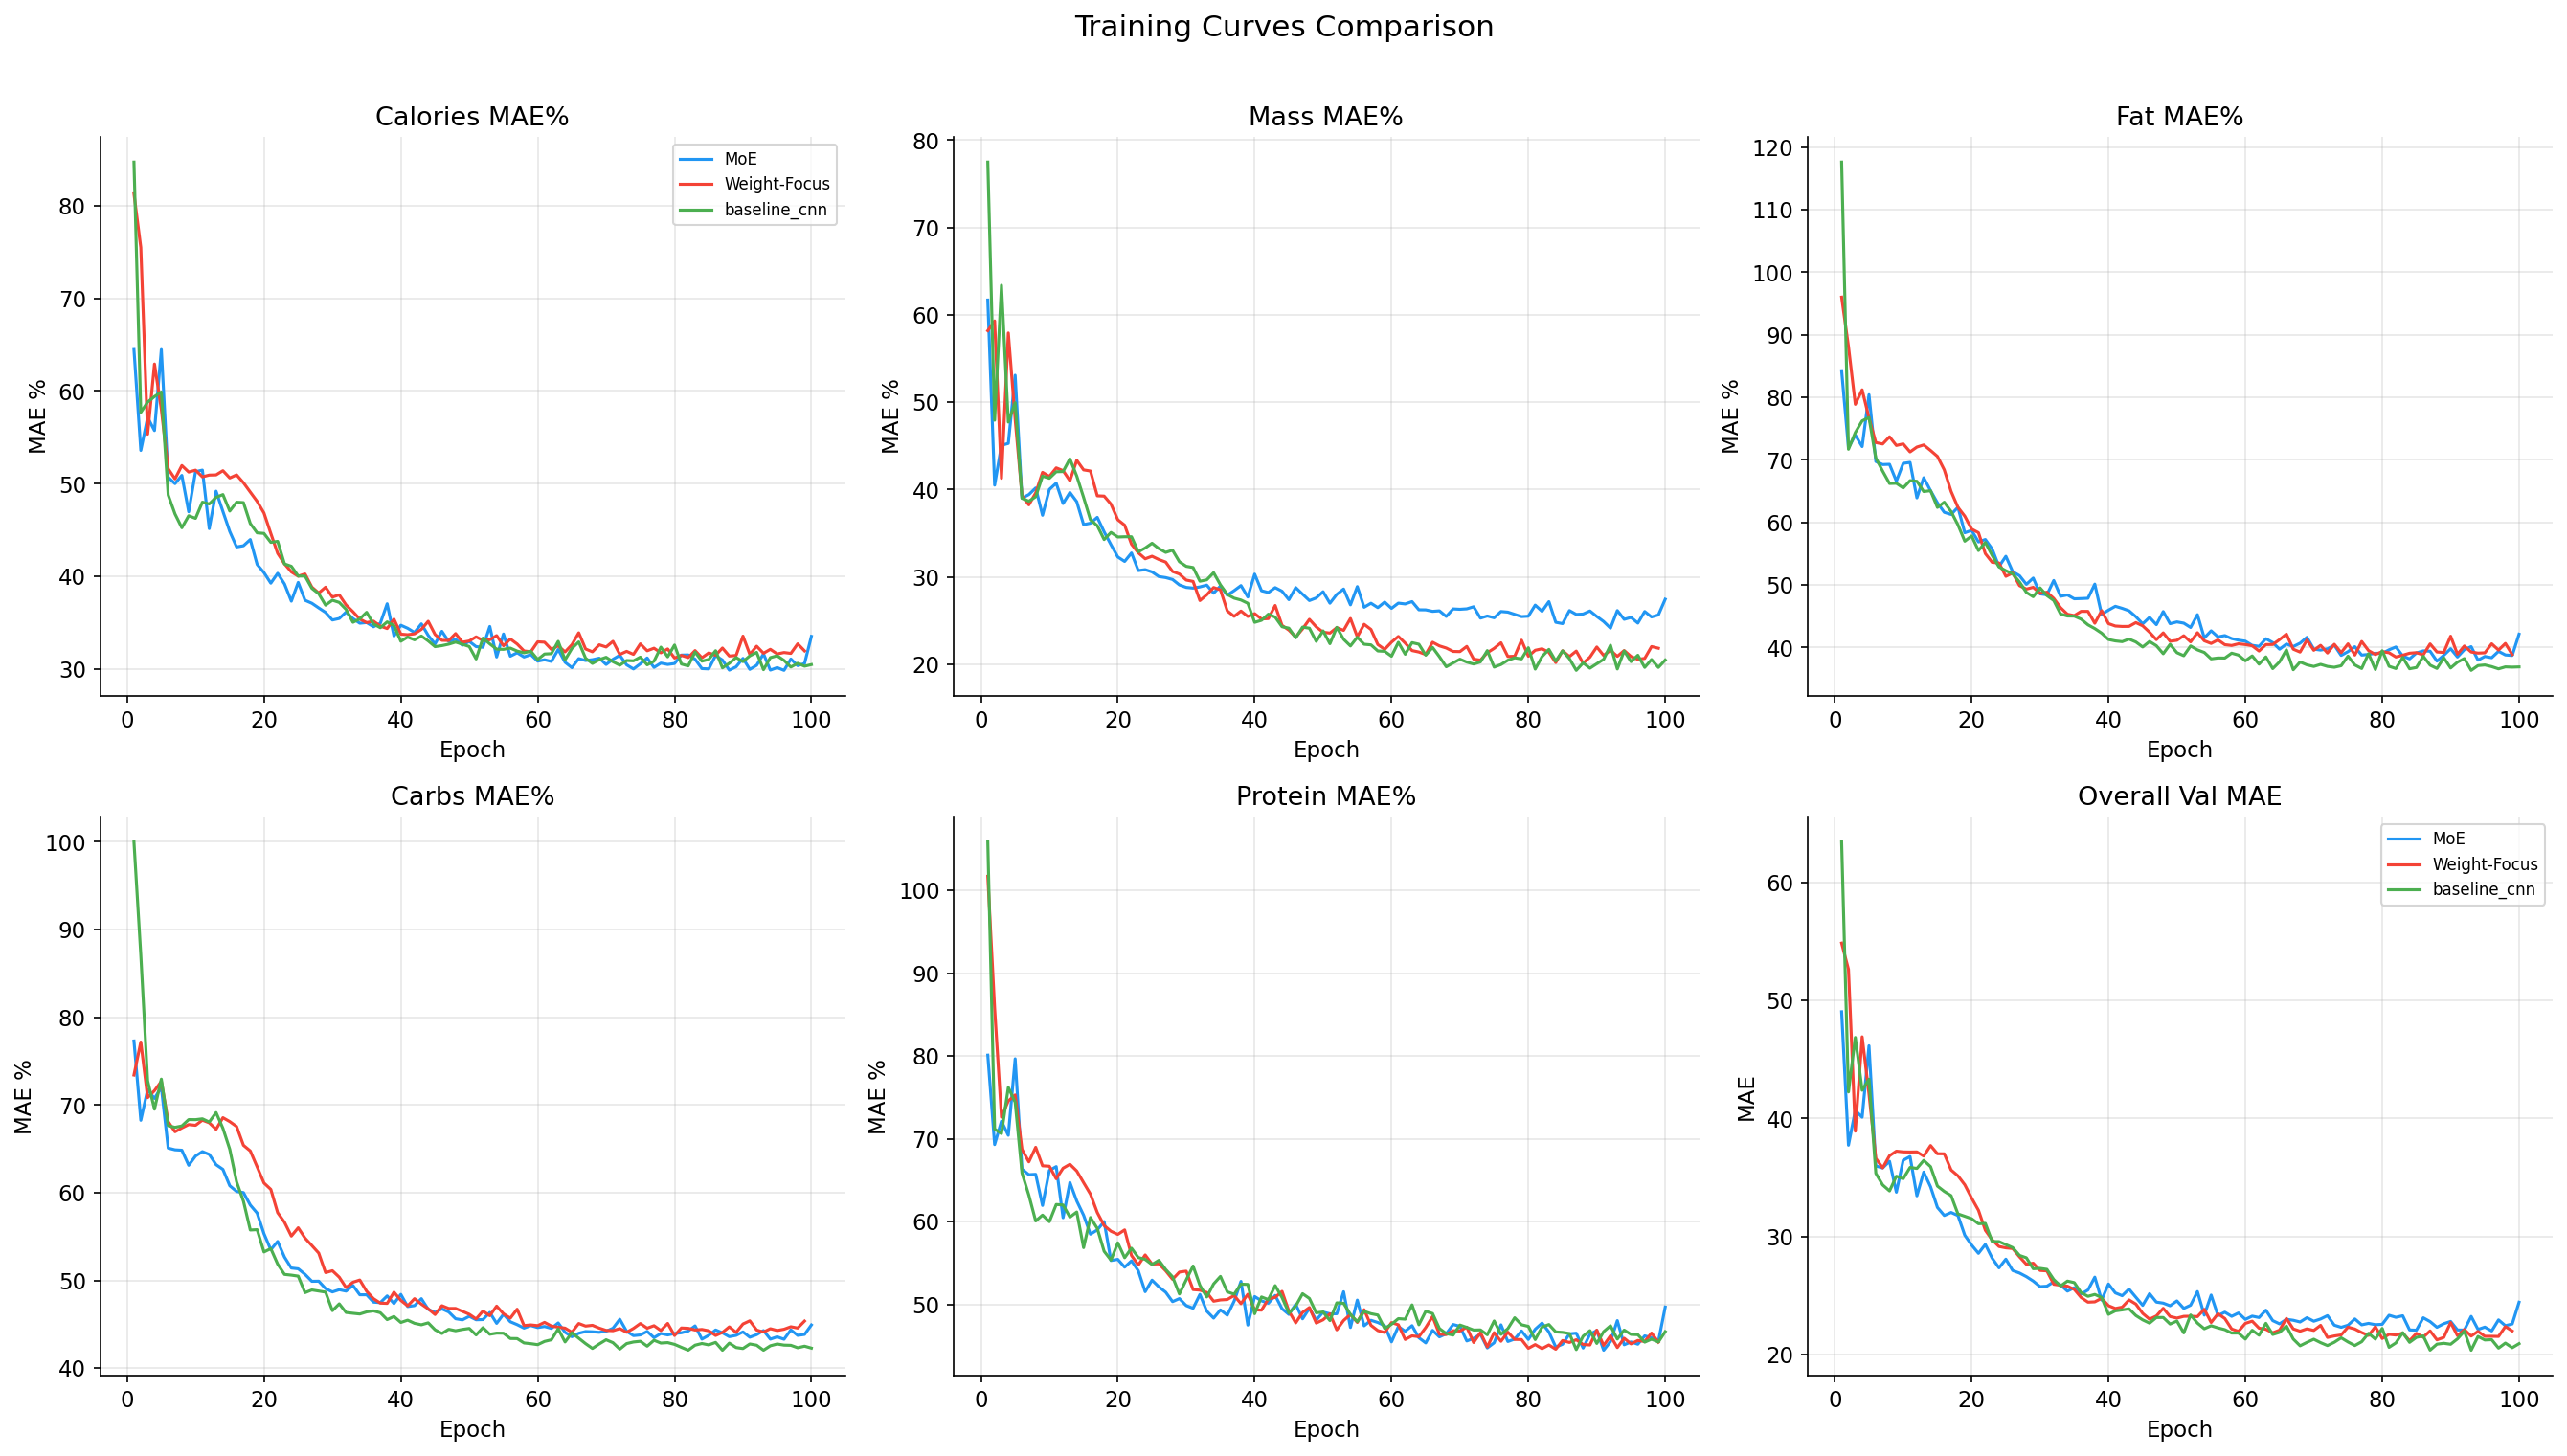
\includegraphics[width=0.85\textwidth]{comparison_training_curves.png}
\caption{Validation MAE over training epochs for all three model variants. The Baseline CNN (blue) consistently achieves the lowest validation MAE after the initial convergence period.}
\label{fig:training_curves}
\end{figure}

\subsection{MAE Comparison by Nutrient}

Figures~\ref{fig:mae_bar} and \ref{fig:mae_pct_bar} show the per-nutrient MAE and MAE\% comparisons across models as bar charts.

\begin{figure}[H]
\centering
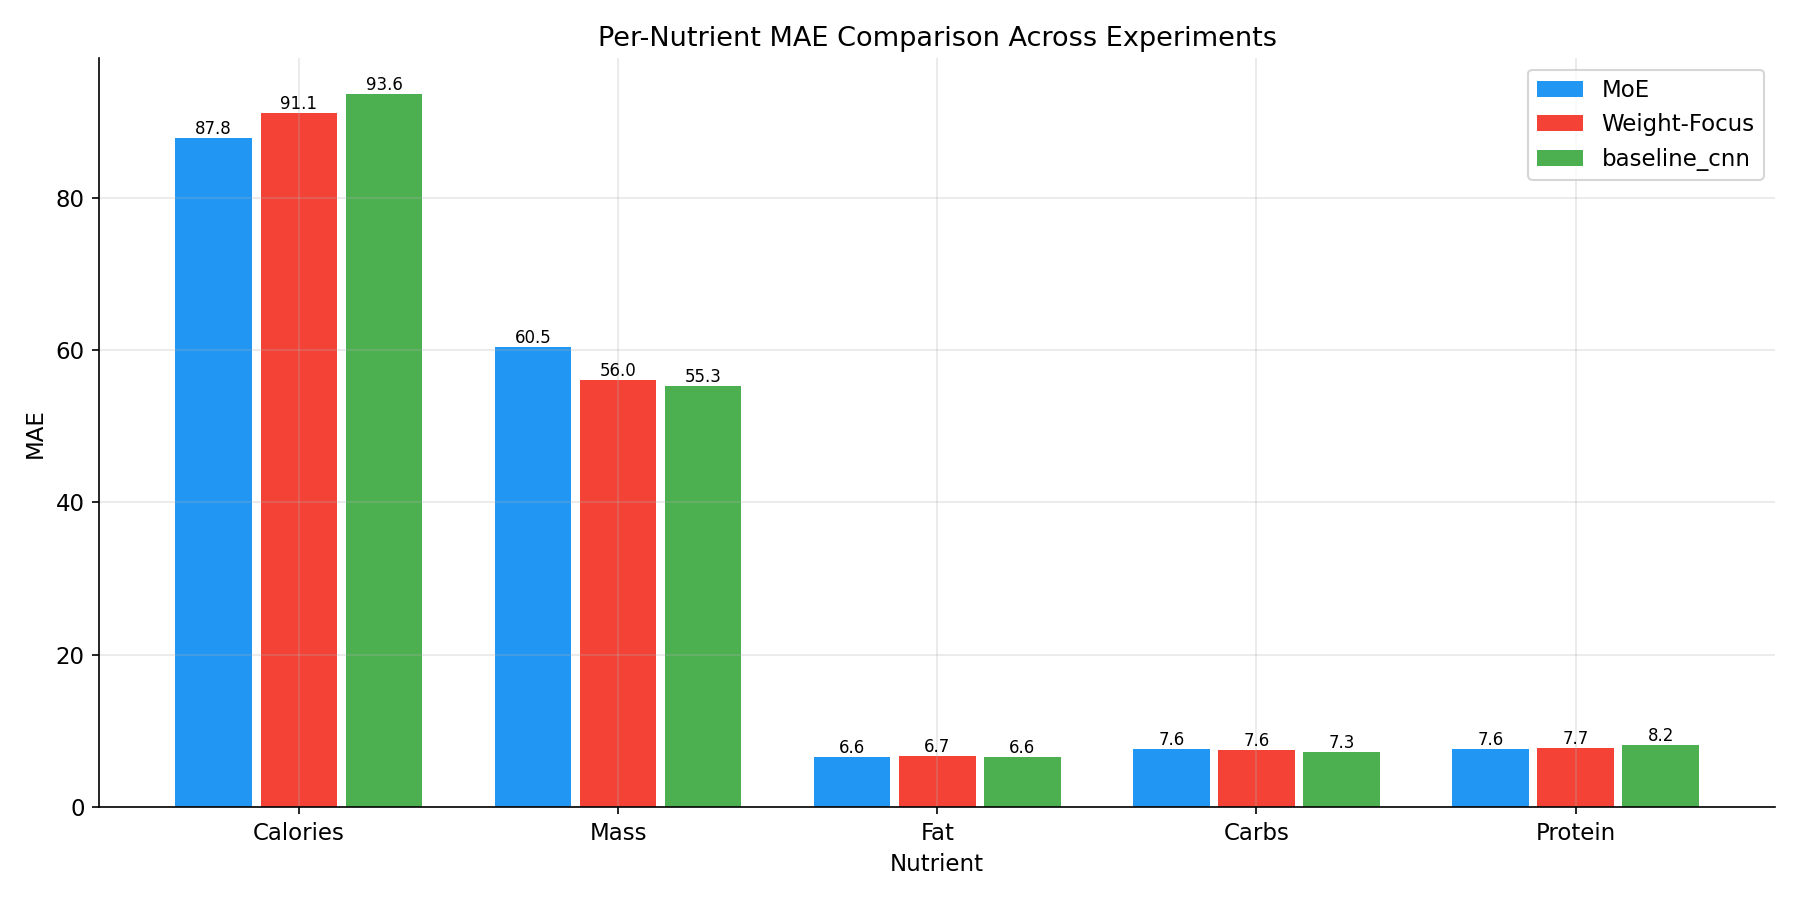
\includegraphics[width=0.85\textwidth]{comparison_mae_bar.png}
\caption{Per-nutrient MAE comparison across the three model variants. The Baseline CNN achieves the lowest MAE for most nutrients.}
\label{fig:mae_bar}
\end{figure}

\begin{figure}[H]
\centering
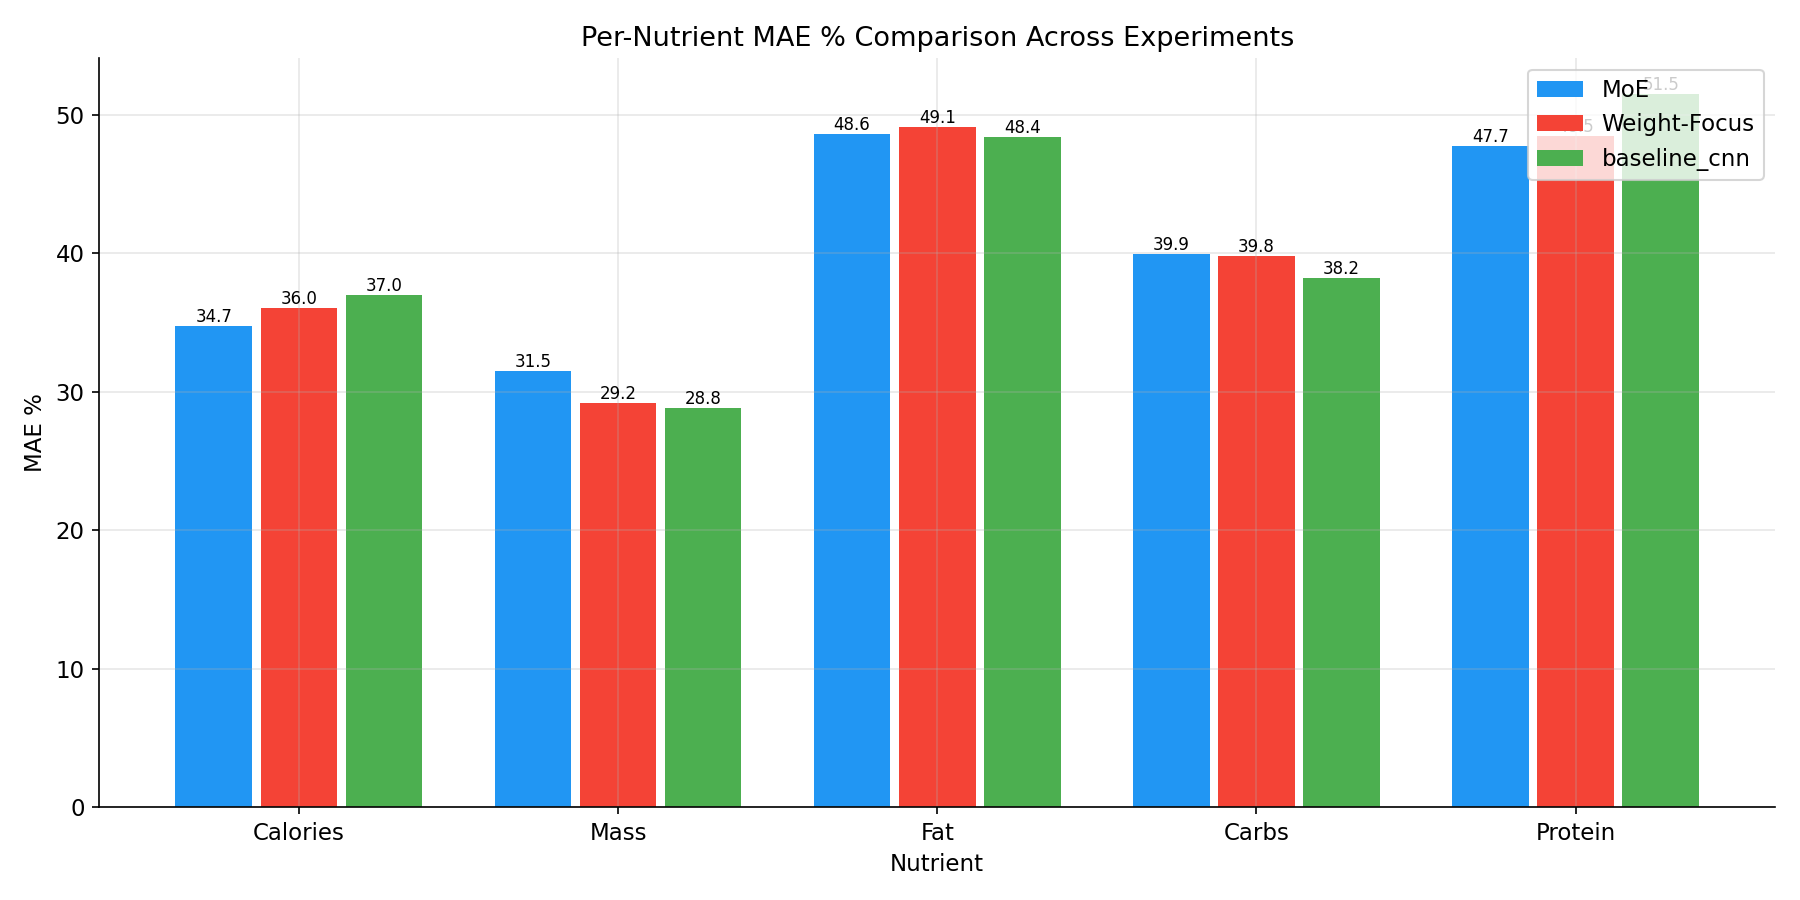
\includegraphics[width=0.85\textwidth]{comparison_mae_pct_bar.png}
\caption{Per-nutrient MAE\% comparison. Lower is better. Mass is the most accurately predicted nutrient across all models.}
\label{fig:mae_pct_bar}
\end{figure}

\subsection{Radar Chart}

Figure~\ref{fig:radar} provides a radar (spider) chart visualization of MAE\% across all five nutrients for each model, making it easy to see the relative strengths and weaknesses at a glance.

\begin{figure}[H]
\centering
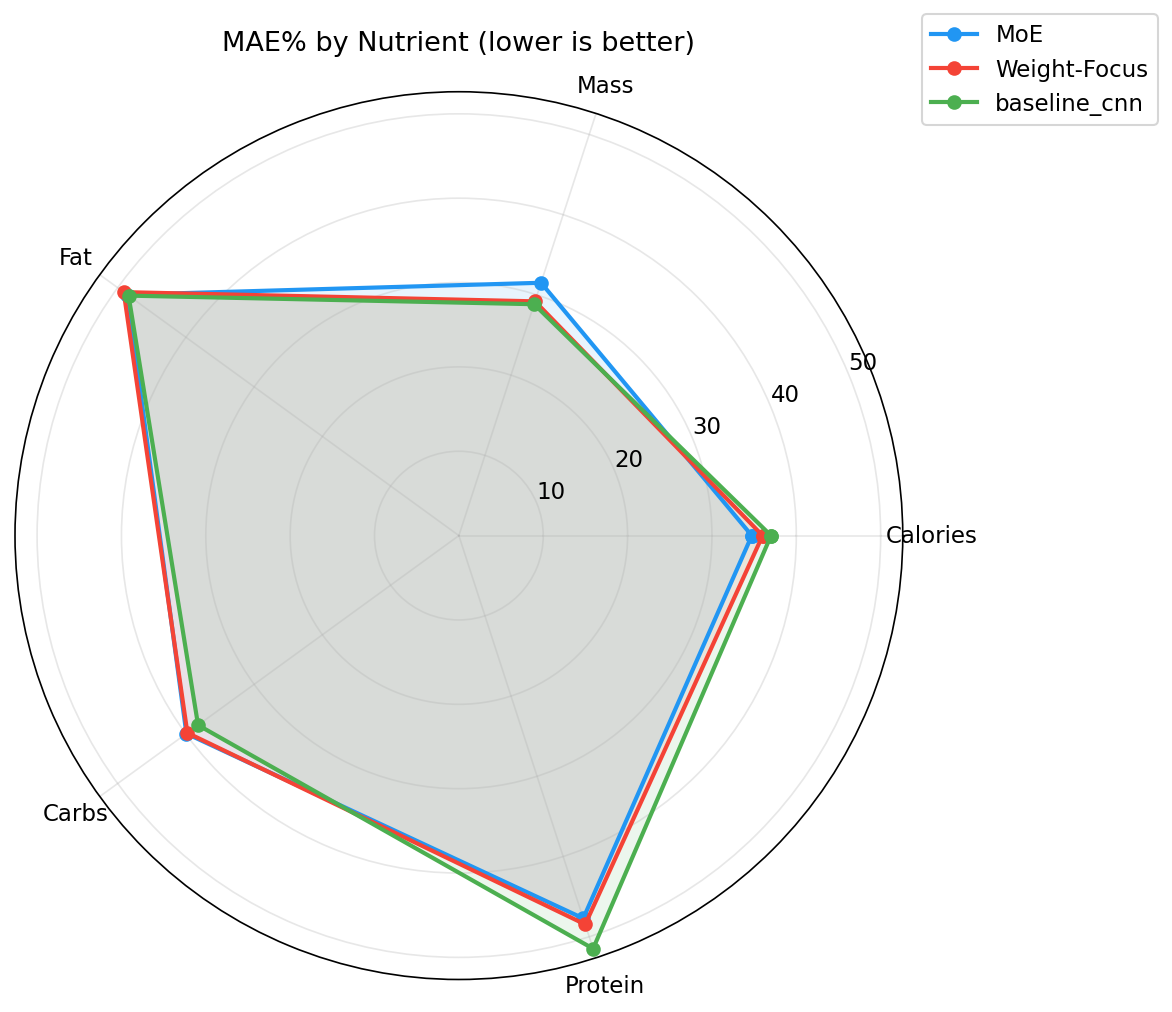
\includegraphics[width=0.7\textwidth]{comparison_radar.png}
\caption{Radar chart of MAE\% across all five nutrients for each model. Smaller area indicates better performance. The Baseline CNN (blue) has the smallest footprint.}
\label{fig:radar}
\end{figure}

\subsection{Prediction Scatter Plots}

Figures~\ref{fig:scatter_calories} and \ref{fig:scatter_mass} show scatter plots of predicted vs.\ ground-truth values for calories and mass, respectively. Points closer to the diagonal indicate more accurate predictions.

\begin{figure}[H]
\centering
\begin{subfigure}[b]{0.48\textwidth}
  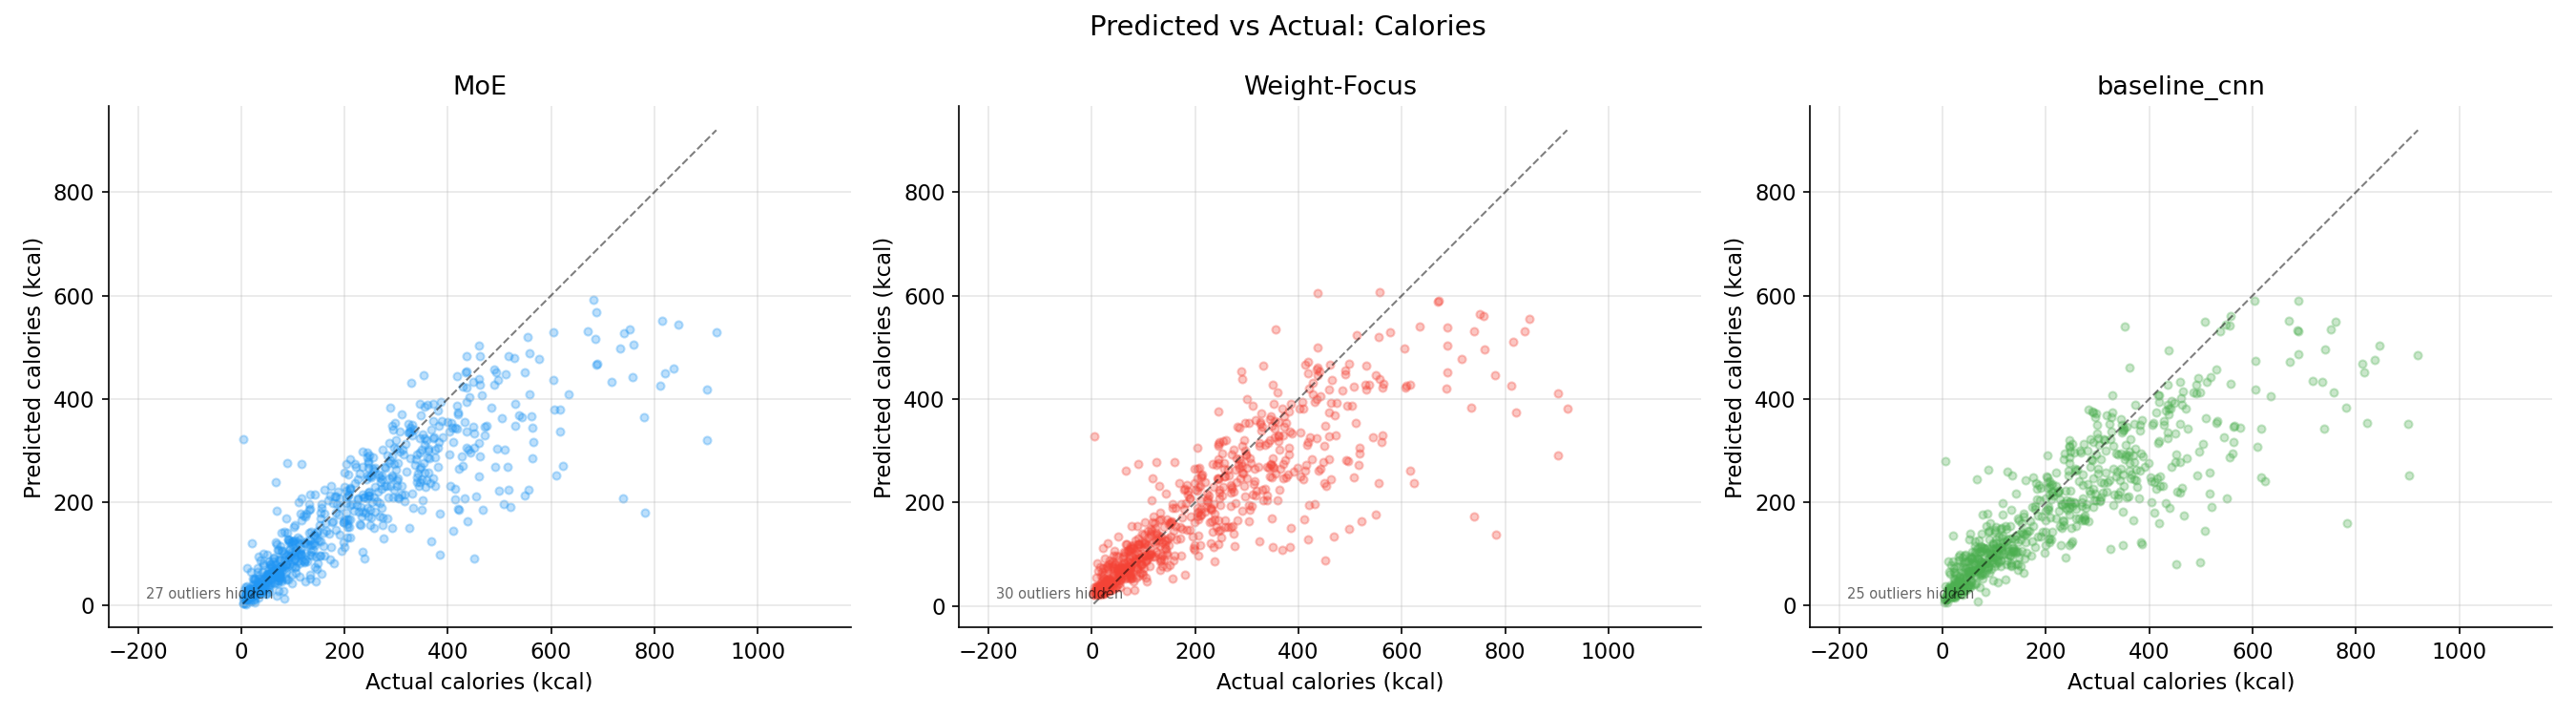
\includegraphics[width=\textwidth]{comparison_scatter_calories.png}
  \caption{Calories}
  \label{fig:scatter_calories}
\end{subfigure}
\hfill
\begin{subfigure}[b]{0.48\textwidth}
  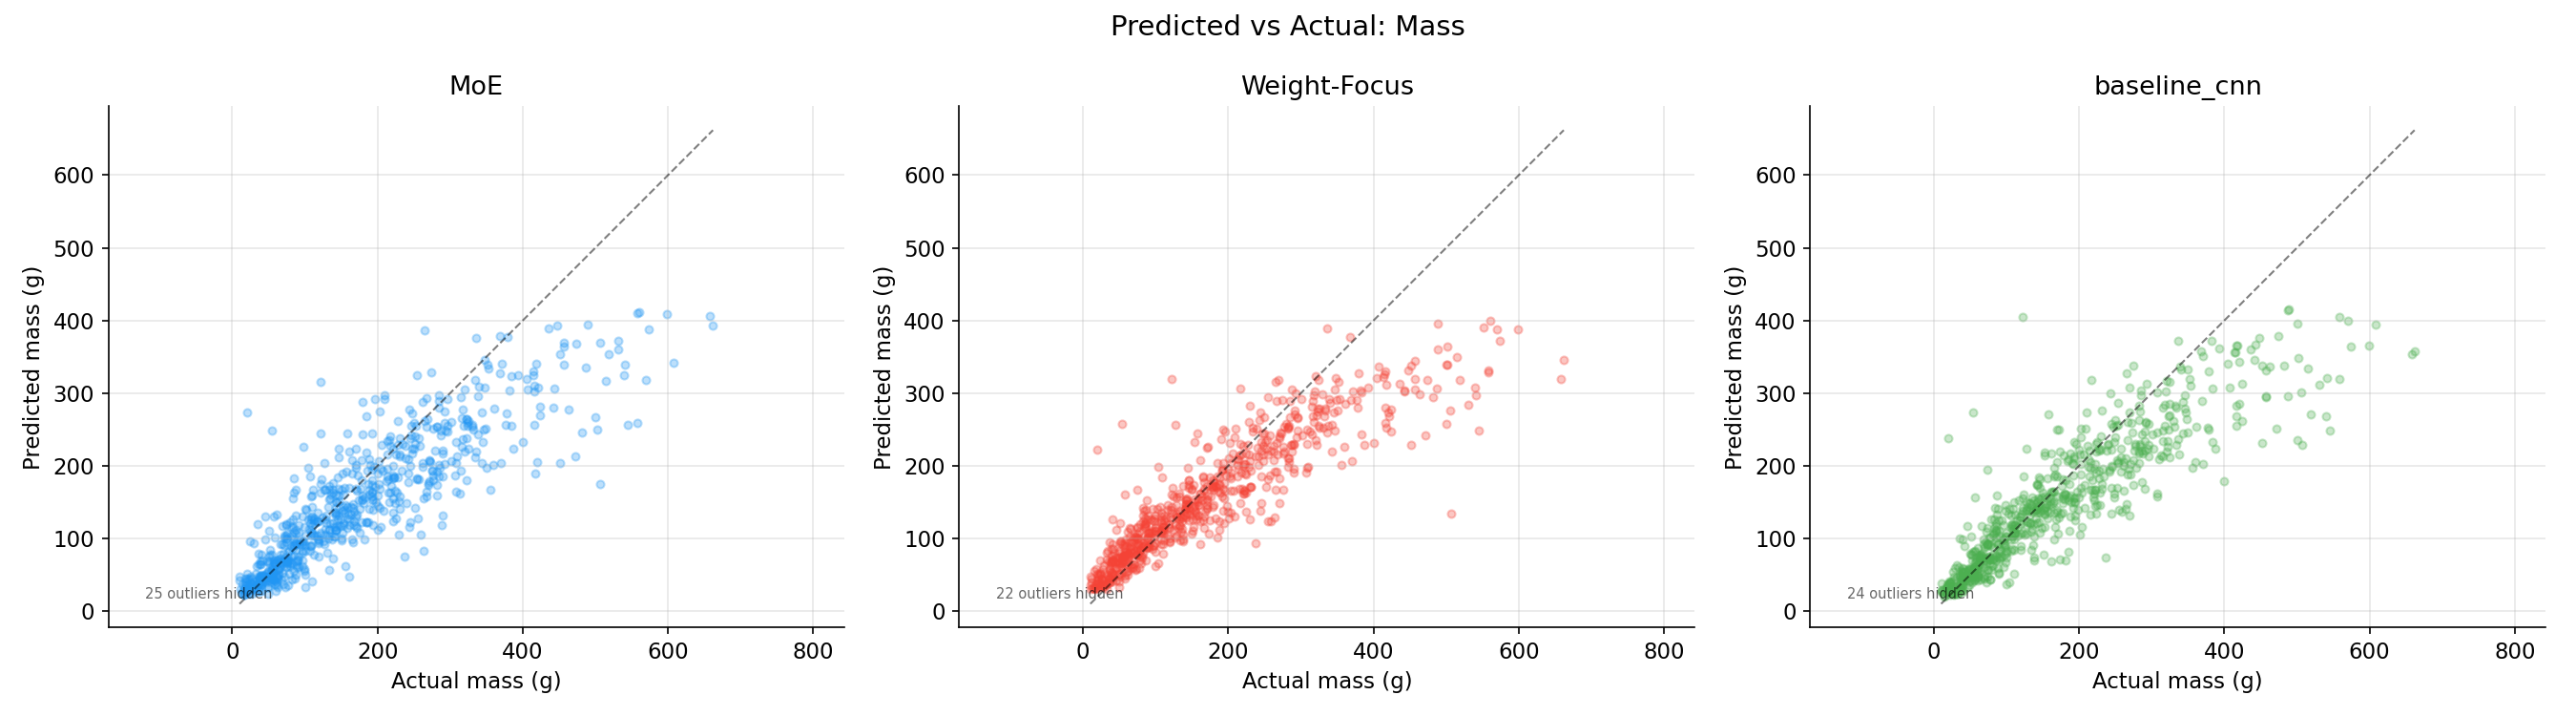
\includegraphics[width=\textwidth]{comparison_scatter_mass.png}
  \caption{Mass}
  \label{fig:scatter_mass}
\end{subfigure}
\caption{Predicted vs.\ ground-truth scatter plots for (a) calories and (b) mass. Points near the diagonal line indicate accurate predictions.}
\label{fig:scatter_plots}
\end{figure}

\subsection{Error Distribution}

Figure~\ref{fig:error_dist} shows the distribution of prediction errors across all nutrients for each model. Tighter, more centered distributions indicate more consistent predictions.

\begin{figure}[H]
\centering
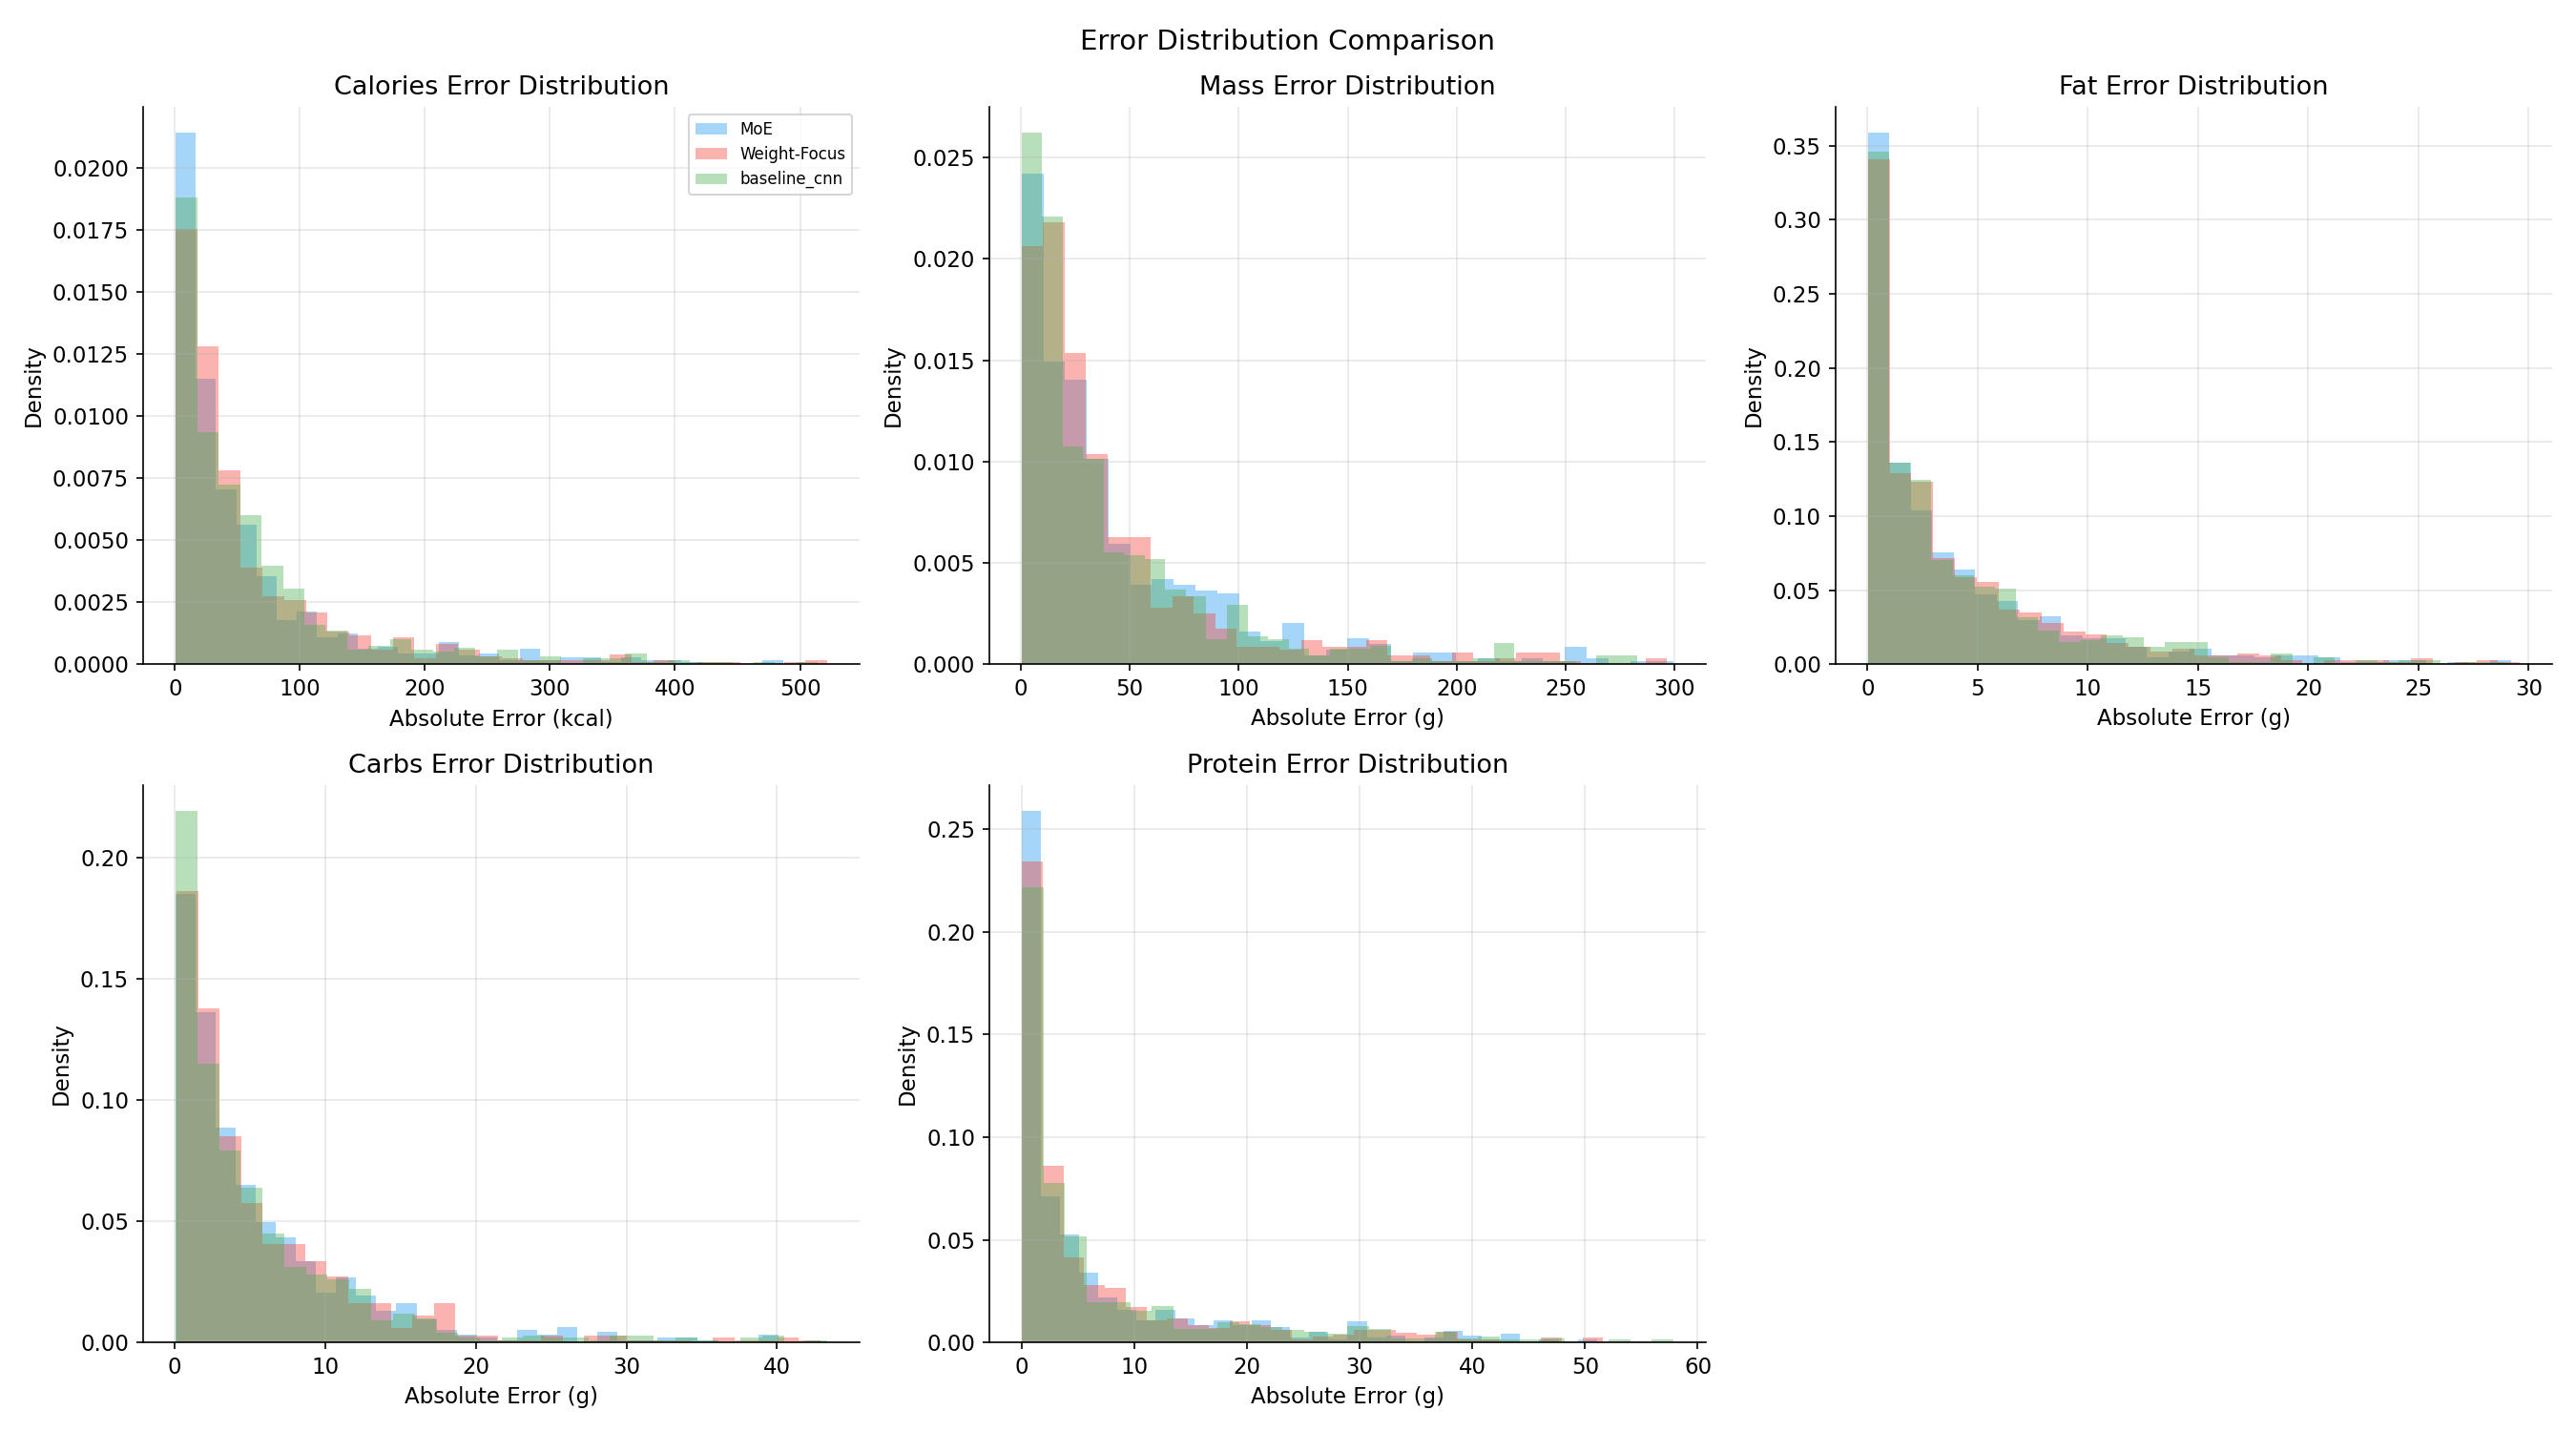
\includegraphics[width=0.85\textwidth]{comparison_error_dist.png}
\caption{Error distribution (predicted $-$ actual) across all nutrients. The Baseline CNN shows the tightest distribution centered around zero.}
\label{fig:error_dist}
\end{figure}

\subsection{Discussion}

\subsubsection{Why Did the Baseline Outperform?}

The most notable finding is that the simplest architecture---the Baseline CNN---achieved the best performance. We attribute this to several factors:

\begin{enumerate}
  \item \textbf{Larger shared representation}: The Baseline and Weight-Focus models use 4096-dimensional shared FC layers, while the MoE model uses 2048-dimensional expert networks. The higher dimensionality provides more capacity for the shared representation, which appears more beneficial than expert specialization for this dataset.

  \item \textbf{Dataset size}: With only $\sim$4,000 unique dishes (9,409 training samples including multiple viewpoints), the dataset may be too small for the MoE model to learn meaningful expert specialization. The gate network may not have enough signal to differentiate between food types.

  \item \textbf{Mass conditioning overhead}: In the Weight-Focus variant, despite the 3$\times$ weighted loss on mass to prioritize its accuracy, errors in the mass prediction still propagate to all other nutrient predictions via the concatenated 4097-dim input. The weighted loss helps mass accuracy but the cascading error amplification appears to negate any benefit from the structural prior.

  \item \textbf{Load-balancing regularization}: The MoE variant includes a balance loss ($\lambda = 0.01$) to prevent expert collapse. While this successfully maintains expert utilization, the additional loss term competes with the primary L1 objective during optimization, potentially distracting the model from learning the best nutritional predictions.

  \item \textbf{Regularization balance}: The larger FC layers in the Baseline model, combined with aggressive dropout ($p = 0.6$), seem to strike a better balance between capacity and regularization than the MoE's smaller 2048-dim experts.
\end{enumerate}

\subsubsection{Per-Nutrient Analysis}

\begin{itemize}
  \item \textbf{Mass} ($\sim$20--27\% MAE\%) was the easiest to predict, likely because food weight has a more direct visual relationship to portion size than other nutrients.
  \item \textbf{Protein} ($\sim$45--50\% MAE\%) was the hardest to predict, possibly because protein content varies widely between food types that may look similar (e.g., chicken vs.\ tofu).
  \item \textbf{Calories} and \textbf{fat} showed moderate predictability ($\sim$30--42\% MAE\%), consistent with the reference paper's findings.
  \item \textbf{Carbohydrates} were difficult to predict ($\sim$42--45\% MAE\%), possibly due to the visual similarity between high-carb and low-carb foods (e.g., white rice vs.\ cauliflower rice).
\end{itemize}

\subsubsection{Comparison with Reference Paper}

The reference paper \cite{thames2021} reported calorie MAE\% of approximately 15--20\% using InceptionV2 pretrained on JFT-300M. Our best model achieves $\sim$30.5\% MAE\% for calories. The performance gap is expected due to:
\begin{itemize}
  \item Using ImageNet pretraining instead of JFT-300M (300M images vs.\ 1.2M)
  \item Using InceptionV3 instead of InceptionV2 (different architecture)
  \item Potential differences in data preprocessing and augmentation strategies
\end{itemize}

% ===========================================================================
% 7. SUMMARY AND CONCLUSIONS
% ===========================================================================
\section{Summary and Conclusions}
\label{sec:conclusion}

In this project, we implemented and compared three deep learning architectures for predicting nutritional content from food images using the Nutrition5k dataset. Our key findings are:

\begin{enumerate}
  \item The \textbf{Baseline CNN}---following the reference paper's architecture with InceptionV3, shared 4096-dim FC layers, and independent task heads---achieved the best performance with an average MAE\% of 35.4\% across all five nutrients.

  \item The \textbf{Weight-Focus} variant, which conditions other nutrient predictions on a mass estimate, did not improve overall performance (MAE\% of 36.7\%). Error propagation from the mass head to conditioned heads likely negated any benefit from the structural prior.

  \item The \textbf{Mixture of Experts} variant, despite its theoretical appeal for learning food-type-specific representations, performed worst (MAE\% of 39.5\%) while using only half the parameters of the other models. The dataset appears too small for effective expert specialization.

  \item \textbf{Transfer learning} with progressive unfreezing was critical for all models, allowing effective fine-tuning of ImageNet features for the nutrition prediction task.

  \item \textbf{Multi-view training} (overhead + side-angle images) significantly increased the effective training set size and provided complementary viewpoint information.
\end{enumerate}

\subsection{Lessons Learned}

\begin{itemize}
  \item Simpler architectures with sufficient capacity can outperform more complex designs, especially on smaller datasets.
  \item Label normalization is essential for multi-task regression with outputs of different scales.
  \item Aggressive dropout ($p = 0.6$) is necessary to prevent overfitting given the relatively small dataset.
  \item The gap between our results and the reference paper highlights the importance of pretraining data (JFT-300M vs.\ ImageNet).
\end{itemize}

\subsection{Future Work}

Several directions could improve upon this work:
\begin{itemize}
  \item \textbf{Larger pretraining}: Using models pretrained on larger datasets (e.g., LAION-5B, OpenImages) or using foundation models (e.g., CLIP, DINOv2) as the backbone.
  \item \textbf{Vision Transformers}: Replacing the CNN backbone with a Vision Transformer (ViT) which may better capture global relationships in food images.
  \item \textbf{Attention mechanisms}: Adding spatial attention to focus on food regions and ignore plate/tray background.
  \item \textbf{Ingredient-level prediction}: Predicting individual ingredient quantities rather than aggregate dish-level nutrition.
  \item \textbf{Larger datasets}: Combining Nutrition5k with other food datasets (e.g., Food-101, Recipe1M) for pretraining.
  \item \textbf{Multi-view fusion}: Developing explicit multi-view fusion strategies (e.g., cross-attention between overhead and side views) rather than treating each view independently.
\end{itemize}

% ===========================================================================
% 8. REFERENCES
% ===========================================================================
\section{References}
\label{sec:references}

\begin{thebibliography}{10}

\bibitem{thames2021}
Q.~Thames, A.~Kar, J.~Carballo, A.~Mottaghi, E.~Edelsbrunner, P.~Joshi, and others,
``Nutrition5k: Towards Automatic Nutritional Understanding of Generic Food,''
in \textit{Proceedings of the IEEE/CVF Conference on Computer Vision and Pattern Recognition (CVPR)}, 2021.
arXiv:2103.03375.

\bibitem{szegedy2016}
C.~Szegedy, V.~Vanhoucke, S.~Ioffe, J.~Shlens, and Z.~Wojna,
``Rethinking the Inception Architecture for Computer Vision,''
in \textit{Proceedings of the IEEE Conference on Computer Vision and Pattern Recognition (CVPR)}, pp.~2818--2826, 2016.

\bibitem{deng2009}
J.~Deng, W.~Dong, R.~Socher, L.-J.~Li, K.~Li, and L.~Fei-Fei,
``ImageNet: A Large-Scale Hierarchical Image Database,''
in \textit{Proceedings of the IEEE Conference on Computer Vision and Pattern Recognition (CVPR)}, pp.~248--255, 2009.

\bibitem{hinton2012}
G.~Hinton, N.~Srivastava, and K.~Swersky,
``Neural Networks for Machine Learning: Lecture 6a --- Overview of Mini-batch Gradient Descent,''
Coursera, 2012.

\bibitem{loshchilov2017}
I.~Loshchilov and F.~Hutter,
``SGDR: Stochastic Gradient Descent with Warm Restarts,''
in \textit{International Conference on Learning Representations (ICLR)}, 2017.

\bibitem{pytorch}
A.~Paszke, S.~Gross, F.~Massa, and others,
``PyTorch: An Imperative Style, High-Performance Deep Learning Library,''
in \textit{Advances in Neural Information Processing Systems (NeurIPS)}, pp.~8024--8035, 2019.

\bibitem{nutrition5k_github}
Google Research,
``Nutrition5k Dataset,''
\url{https://github.com/google-research/google-research/tree/master/nutrition5k}, 2021.

\end{thebibliography}

% ===========================================================================
% 9. APPENDIX — CODE LISTINGS
% ===========================================================================
\newpage
\appendix
\section{Appendix: Code Listings}
\label{sec:appendix}

Full source code is available in the \texttt{Code/} directory of the GitHub repository: \url{https://github.com/ZacBland/Final-Project-ZacBland}.

\subsection{Baseline Model Architecture (\texttt{Code/train.py})}

\begin{lstlisting}[caption={NutritionModel class --- Baseline CNN architecture.}]
class NutritionModel(nn.Module):
    """
    InceptionV3 backbone with multi-task regression head.
    backbone features -> shared 2x FC(4096) -> per-task FC(4096) -> FC(1) x 5
    """
    def __init__(self, num_tasks=5, dropout=0.6):
        super().__init__()
        self.backbone = models.inception_v3(
            weights=models.Inception_V3_Weights.IMAGENET1K_V1,
            aux_logits=True,
        )
        self.backbone.aux_logits = False
        self.backbone.AuxLogits = None
        self.backbone.fc = nn.Identity()

        self.shared = nn.Sequential(
            nn.Flatten(),
            nn.Linear(2048, 4096),
            nn.ReLU(inplace=True),
            nn.Dropout(dropout),
            nn.Linear(4096, 4096),
            nn.ReLU(inplace=True),
            nn.Dropout(dropout),
        )

        self.task_heads = nn.ModuleList([
            nn.Sequential(
                nn.Linear(4096, 4096),
                nn.ReLU(inplace=True),
                nn.Dropout(dropout),
                nn.Linear(4096, 1),
            )
            for _ in range(num_tasks)
        ])

    def forward(self, x):
        features = self.backbone(x)
        shared_out = self.shared(features)
        outputs = [head(shared_out) for head in self.task_heads]
        return torch.cat(outputs, dim=1)
\end{lstlisting}

\subsection{Weight-Focus Model Architecture (\texttt{weight-focus} branch)}

\begin{lstlisting}[caption={NutritionModel class --- Weight-Focus architecture with mass-conditioned heads.}]
class NutritionModel(nn.Module):
    """
    Mass-conditioned multi-task regression head.
    backbone -> shared 2x FC(4096) -> mass head -> mass_pred
                                    -> 4 conditioned heads (shared + mass_pred)
    """
    MASS_IDX = 1  # index of mass in output tensor
    OTHER_IDXS = [0, 2, 3, 4]  # calories, fat, carbs, protein

    def __init__(self, num_tasks=5, dropout=0.6):
        super().__init__()
        self.backbone = models.inception_v3(
            weights=models.Inception_V3_Weights.IMAGENET1K_V1,
            aux_logits=True)
        self.backbone.aux_logits = False
        self.backbone.AuxLogits = None
        self.backbone.fc = nn.Identity()

        self.shared = nn.Sequential(
            nn.Flatten(),
            nn.Linear(2048, 4096), nn.ReLU(inplace=True), nn.Dropout(dropout),
            nn.Linear(4096, 4096), nn.ReLU(inplace=True), nn.Dropout(dropout))

        # Mass head: predicted independently
        self.mass_head = nn.Sequential(
            nn.Linear(4096, 4096), nn.ReLU(inplace=True),
            nn.Dropout(dropout), nn.Linear(4096, 1))

        # Conditioned heads: input is 4097 = 4096 shared + 1 mass pred
        self.conditioned_heads = nn.ModuleList([
            nn.Sequential(
                nn.Linear(4097, 4096), nn.ReLU(inplace=True),
                nn.Dropout(dropout), nn.Linear(4096, 1))
            for _ in range(num_tasks - 1)])

    def forward(self, x):
        features = self.backbone(x)
        shared_out = self.shared(features)
        mass_pred = self.mass_head(shared_out)           # (B, 1)
        cond_input = torch.cat([shared_out, mass_pred], dim=1)  # (B, 4097)
        cond_preds = [head(cond_input) for head in self.conditioned_heads]
        outputs = [None] * 5
        outputs[self.MASS_IDX] = mass_pred
        for i, idx in enumerate(self.OTHER_IDXS):
            outputs[idx] = cond_preds[i]
        return torch.cat(outputs, dim=1)                 # (B, 5)
\end{lstlisting}

The Weight-Focus training loop uses a weighted per-task loss:
\begin{lstlisting}[caption={Weighted loss computation in Weight-Focus training.}]
TASK_WEIGHTS = [1.0, 3.0, 1.0, 1.0, 1.0]  # prioritize mass prediction

# In train_one_epoch():
tw = torch.tensor(TASK_WEIGHTS, dtype=torch.float32).to(device)
loss = ((preds - norm_labels).abs() * tw).mean()
\end{lstlisting}

\subsection{Mixture of Experts Model Architecture (\texttt{MoE} branch)}

\begin{lstlisting}[caption={NutritionModel class --- Mixture of Experts architecture.}]
class NutritionModel(nn.Module):
    """
    MoE multi-task regression.
    backbone (2048) -> gate (softmax over N experts)
                    -> N expert networks (2048->2048->2048)
                    -> weighted sum -> per-task heads (2048->1024->1) x 5
    forward() returns (predictions, balance_loss).
    """
    def __init__(self, num_tasks=5, num_experts=4, dropout=0.6):
        super().__init__()
        self.num_experts = num_experts
        self.backbone = models.inception_v3(
            weights=models.Inception_V3_Weights.IMAGENET1K_V1,
            aux_logits=True)
        self.backbone.aux_logits = False
        self.backbone.AuxLogits = None
        self.backbone.fc = nn.Identity()

        self.gate = nn.Sequential(
            nn.Flatten(), nn.Linear(2048, num_experts),
            nn.Softmax(dim=1))

        self.experts = nn.ModuleList([
            nn.Sequential(
                nn.Flatten(),
                nn.Linear(2048, 2048), nn.ReLU(inplace=True), nn.Dropout(dropout),
                nn.Linear(2048, 2048), nn.ReLU(inplace=True), nn.Dropout(dropout))
            for _ in range(num_experts)])

        self.task_heads = nn.ModuleList([
            nn.Sequential(
                nn.Linear(2048, 1024), nn.ReLU(inplace=True),
                nn.Dropout(dropout), nn.Linear(1024, 1))
            for _ in range(num_tasks)])

    def forward(self, x):
        features = self.backbone(x)
        gate_weights = self.gate(features)               # (B, num_experts)
        expert_outs = torch.stack(
            [e(features) for e in self.experts], dim=1)  # (B, num_experts, 2048)
        combined = (gate_weights.unsqueeze(-1) * expert_outs).sum(dim=1)
        outputs = [head(combined) for head in self.task_heads]
        preds = torch.cat(outputs, dim=1)
        # Load-balancing loss
        importance = gate_weights.mean(dim=0)
        balance_loss = self.num_experts * (importance ** 2).sum()
        return preds, balance_loss
\end{lstlisting}

The MoE training loop adds the balance loss to the primary L1 loss:
\begin{lstlisting}[caption={MoE training step with balance loss.}]
BALANCE_LOSS_WEIGHT = 0.01

# In train_one_epoch():
preds, balance_loss = model(images)
loss = criterion(preds, norm_labels) + BALANCE_LOSS_WEIGHT * balance_loss
\end{lstlisting}

\subsection{Dataset Class (\texttt{Code/train.py})}

\begin{lstlisting}[caption={Nutrition5kDataset --- Custom dataset for multi-view food images.}]
class Nutrition5kDataset(Dataset):
    """Dataset for Nutrition5k images (overhead + optional side-angle)."""
    def __init__(self, data_dir, split_file=None, dish_ids=None,
                 transform=None, side_angle_transform=None,
                 max_dishes=None, image_sources=None,
                 side_cameras=None, max_side_frames=None):
        self.data_dir = data_dir
        self.transform = transform
        self.side_angle_transform = side_angle_transform or transform

        if image_sources is None:
            image_sources = ["overhead"]

        # Load split IDs from file or list
        if dish_ids is not None:
            split_ids = list(dish_ids)
        elif split_file is not None:
            split_path = os.path.join(data_dir, split_file)
            with open(split_path, "r") as f:
                split_ids = [line.strip() for line in f if line.strip()]

        metadata = load_metadata(data_dir)
        self.samples = []

        for dish_id in split_ids:
            if dish_id not in metadata:
                continue
            labels = metadata[dish_id]
            if "overhead" in image_sources:
                img_path = os.path.join(
                    data_dir, "imagery", "realsense_overhead",
                    dish_id, "rgb.png")
                if os.path.exists(img_path):
                    self.samples.append(
                        (img_path, labels, dish_id, "overhead"))
            if "side_angles" in image_sources:
                for camera in side_cameras:
                    frames_dir = os.path.join(
                        data_dir, "imagery", "side_angles",
                        dish_id, camera)
                    if os.path.isdir(frames_dir):
                        frame_files = sorted(glob.glob(
                            os.path.join(frames_dir, "*.png")))
                        for frame_path in frame_files:
                            self.samples.append(
                                (frame_path, labels, dish_id, "side"))

    def __getitem__(self, idx):
        img_path, labels, dish_id, source_type = self.samples[idx]
        image = Image.open(img_path).convert("RGB")
        if source_type == "side" and self.side_angle_transform:
            image = self.side_angle_transform(image)
        elif self.transform:
            image = self.transform(image)
        labels = torch.tensor(labels, dtype=torch.float32)
        return image, labels, dish_id
\end{lstlisting}

\subsection{Training Loop (\texttt{Code/train.py})}

\begin{lstlisting}[caption={Main training loop with progressive unfreezing and early stopping.}]
# Progressive unfreezing
if epoch == FREEZE_BACKBONE_EPOCHS + 1:
    for param in model.backbone.parameters():
        param.requires_grad = True
    optimizer = torch.optim.RMSprop(
        model.parameters(),
        lr=LEARNING_RATE * 0.01,
        weight_decay=WEIGHT_DECAY)
    scheduler = torch.optim.lr_scheduler.CosineAnnealingLR(
        optimizer, T_max=EPOCHS - FREEZE_BACKBONE_EPOCHS)

# Training step
train_loss, train_mae = train_one_epoch(
    model, train_loader, optimizer, criterion,
    device, epoch, EPOCHS, label_mean=label_mean)
val_loss, val_mae, val_mae_pct = validate(
    model, val_loader, criterion, device,
    label_mean=label_mean)
scheduler.step()

# Early stopping
if val_mae_avg < best_val_loss:
    best_val_loss = val_mae_avg
    epochs_without_improvement = 0
    torch.save({...}, checkpoint_path)
else:
    epochs_without_improvement += 1
    if epochs_without_improvement >= EARLY_STOP_PATIENCE:
        break
\end{lstlisting}

\end{document}
